\textgreek{
    Η υλοποίηση έγινε χρησιμοποιώντας δεδομένα επιχειρήσεων απο το
}
Yelp dataset \\ https://www.yelp.com/dataset/challenge

\textgreek{
    Παρακάτω παρουσιάζονται τα βήματα που έγιναν για την προεπεξεργασία
    των δεδομένων.
}

\subsection{\textgreek{Βάση δεδομένων}}
\textgreek{
    Με στόχο την καλύτερη και ευκολότερη διαχείρηση των δεδομένων σε μια
    πιο δομημένη μορφή, δημιουργήθηκε σχεσιακή βάση δεδομένων.

    Το σύστημα διαχείρησης της βάσης δεδομένων που χρησιμοποιήθηκε
    είναι $Postgres$. Το σχήμα που δημιουργήθηκε φαίνεται παρακάτω.

    \begin{center}
        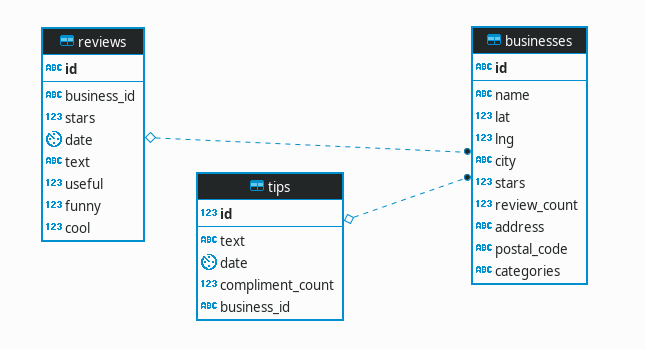
\includegraphics[width=130mm]{media/schema.png}
    \end{center}
}

\subsection{\textgreek{Εισαγωγή δεδομένων}}
\textgreek{
    Η αρχική μορφή των δεδομένων ήταν τύπου $json$.
    Τα δεδομένα μετατράπηκαν
    σε μορφή τύπου $csv$, με σκοπό την ταχύτερη εισαγωγή τους στη βάση δεδομένων.

    Για τη μετατροπή χρησιμοποιήθηκε το πρόγραμμα $jq$.
    Το $script$ για την
    \\ μετατροπή είναι το $src/main/resources/json\_to\_csv.sh$

    Έπειτα για την εισαγωγή των δεδομένων απο τα $csv$ αρχεία χρησιμοποιήθηκαν
    εντολές τύπου $COPY$, για παράδειγμα για τον πίνακα των επιχειρήσεων:
} \\
\texttt{COPY businesses FROM '/path/to/businesses.tsv' DELIMITER '\textbackslash t'}

\subsection{\textgreek{Στατιστικά δεδομένων}}
\textgreek{
    Στην παρούσα φάση όλα τα δεδομένα έχουν εισαχθεί στην βάση δεδομένων,
    με κατάλληλα ερωτήματα $SQL$ μπορούμε να βγάλουμε χρήσιμα στατιστικά
    προκειμένου να γίνει καλύτερη κατανόηση των δεδομένων μας.
}

\paragraph{\textgreek{Στατιστικά πόλεων}}
\textgreek{
    Σε αυτό το βήμα φαίνονται μερικά χρήσιμα στατιστικά ανα πόλη.

    \begin{enumerate}
        \item \textgreek{Αριθμός επιχειρήσεων ανά πόλη.}
        \item \textgreek{Αριθμός κριτικών ανά πόλη.}
        \item \textgreek{Μέσος αριθμός κριτικών και υποδείξεων.}
        \item \textgreek{Αριθμός υποδείξεων ($tips$) ανά πόλη.}
    \end{enumerate}

    \begin{center}
        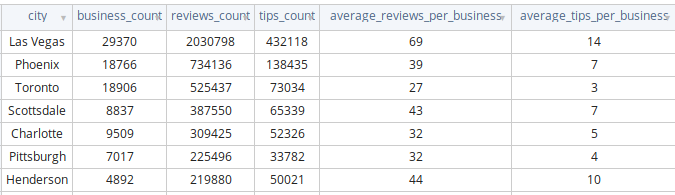
\includegraphics[width=130mm]{media/stats_table.png}
        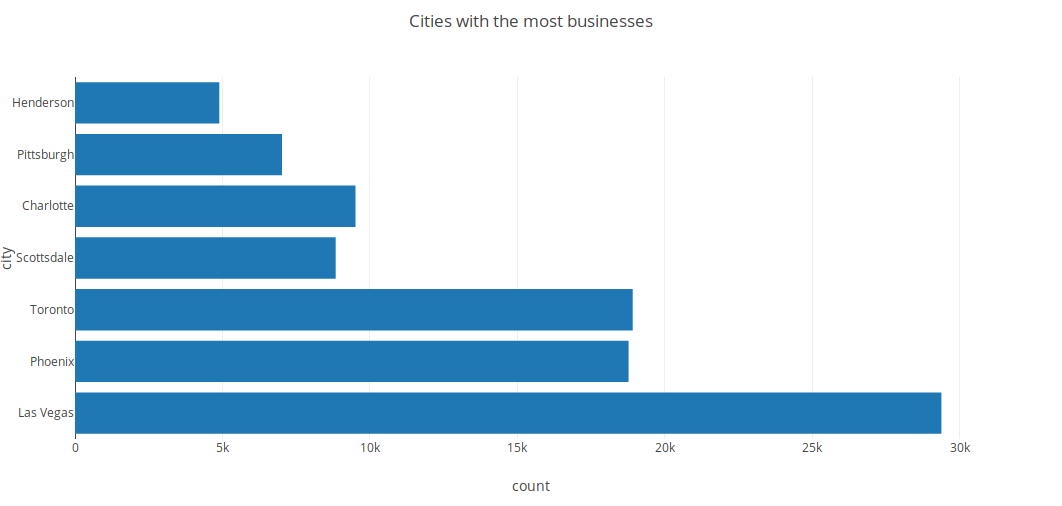
\includegraphics[width=130mm]{media/business_count_chart.png}
        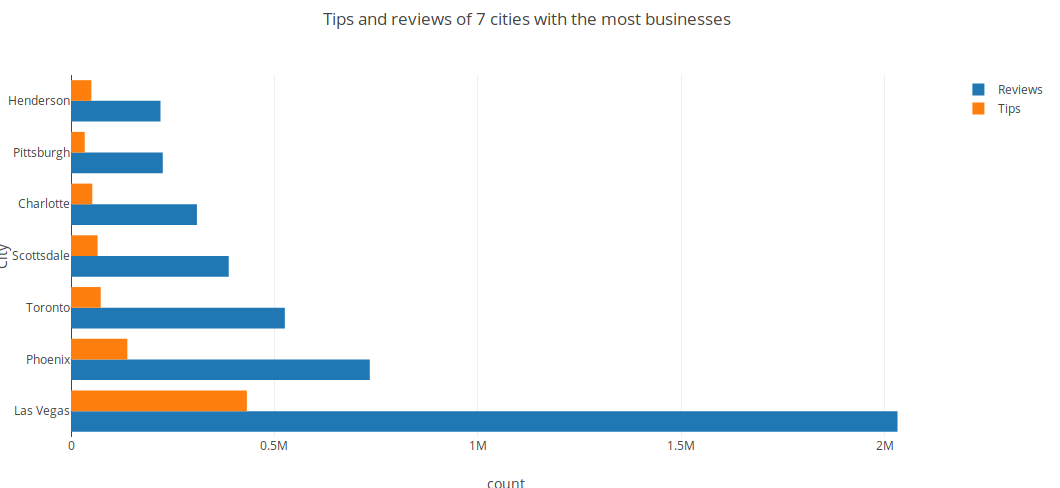
\includegraphics[width=130mm]{media/reviews_and_tips_chart.png}
    \end{center}
}


\subsection{\textgreek{Φιλτράρισμα}}
\textgreek{
    Σε αυτήν την περίπτωση, μπορούμε να εντοπίσουμε παράγοντες
    θορύβου, όπως για παράδειγμα ανεπιθύμητες ($spam$) κριτικές και υποδείξεις
    καθώς και μη έγκυρες επιχειρήσεις.

    Οι επιχειρήσεις και οι κριτικές που δεν περνάνε κατά το στάδιο του
    φιλτραρίσματος, μένουν στην βάση δεδομένων παρόλα αυτά δεν 
    χρησιμοποιούνται κατά την ευρετηρίαση και άρα δεν εμφανίζονται και 
    δεν λαμβάνονται υπόψιν στα αποτελέσματα.

    \begin{enumerate}
        \item \textgreek{Φιλτράρισμα πόλεων.\\
        Η μηχανή αναζήτησης πρέπει να λαμβάνει υπόψιν επιχειρήσεις μόνο
        μίας πόλης, για τον λόγο αυτό θα χρησιμοποιηθεί η πόλη με τις
        περισσότερες επιχειρήσεις.}
        \item \textgreek{Εντοπισμός ανεπιθύμητων ($spam$) κριτικών και υποδέιξεων.\\
        Ο εντοπισμός γίνεται με βάση τον αριθμό λέξεων, το μήκος λέξεων καθώς και
        την συχνότητα εμφάνισης των λέξεων.}
        \item \textgreek{Εντοπισμός μη έγκυρων επιχειρήσεων.\\
        Μη έγκυρες μπορούν να θεωρηθούν επιχειρήσεις με μη επιτρεπτό όνομα,
        ελλειπή στοιχεία, κτλπ.}
    \end{enumerate}
}

\newpage
\subsection{\textgreek{Ευρετηρίαση}}
    \textgreek{
        Κατά την ευρετηρίαση θα δημιουργηθούν τρία ευρετήρια, ένα για κάθε πίνακα.
    }

    \paragraph{\textgreek{Επιχειρήσεις}} {
        \textgreek{
            Κάθε επιχείρηση είναι ένα έγγραφο, τα πεδία που χρησιμοποιούνται
            κατά την ευρετηρίαση των επιχειρήσεων, είναι το αναγνωριστικό καθώς
            και το όνομα τους. Το όνομα χρησιμοποιείται κατά την αναζήτηση, ενώ
            το αναγνωριστικό για την ανάκτηση λοιπών πληροφοριών για την επιχείρηση.
        }
    }

    \paragraph{\textgreek{Κριτικές και υποδείξεις}} {
        \textgreek{
            Κάθε κριτική και υπόδειξη αποτελείται απο ένα έγγραφο. Τα πεδία
            που χρησιμοποιούνται κατά την ευρετηρίαση είναι το αναγνωριστικό
            της επιχείρησης καθώς και το κείμενο απο το οποίο αποτελούνται.
            Το κείμενο χρησιμοποιείται κατά την αναζήτηση, ενώ το
            αναγνωριστικό για την ανάκτηση λοιπών πληροφοριών για την επιχείρηση.
        }
    \paragraph{\textgreek{Ευρετηρίαση Αρχείων}}{
        \textgreek{
            Η ευρετηρίαση των αρχείων γίνεται μία φορά. Με την χρήση των μεθόδων της
            $Lucene$ αποθηκεύουμε τα ανεστραμμένα ευρετήρια που δημιουργούνται στον δίσκο.
            \newline Χρησιμοποιούμε τον $StandardAnalyser$ της $Lucene$ για το $tokenizing$ των εγγράφων μας
            καθώς απαλλείφει $stop-words$ και λευκούς χαρακτήρες.
        }
    }
}
